\chapter{KIẾN THỨC HỆ THỐNG}

\section{Cơ sở lý thuyết của kiến trúc}

\subsection{Kiến trúc Onion}

Onion Architecture (Kiến trúc củ hành) được xây dựng dựa trên ý tưởng đặt Domain vào trung tâm ứng dụng, mở rộng cơ chế phân phối (UI) và cơ sở hạ tầng được xây dựng bởi hệ thống.

Các tầng được biểu diễn thành dạng các vòng tròn đồng tâm. Đặc trưng của kiến trúc củ hành đó là một luật về sự ràng buộc giữa các tầng. Tầng bên ngoài chỉ phụ thuộc và gọi trực tiếp tầng bên trong. Các tầng thấp hơn không thể phụ thuộc vào các tầng bên ngoài.

Hầu hết các kiến trúc truyền thống đều nêu lên những vấn đề cơ bản về sự kết hợp giữa các thành phần một cách chặt chẽ và tách biệt. Kiến trúc Onion được Jeffrey Palermo giới thiệu để cung cấp một cách tốt hơn để xây dựng các ứng dụng theo quan điểm về khả năng kiểm tra, khả năng bảo trì và độ tin cậy tốt hơn.

\subsubsection{Nguyên lý}

Kiến trúc Onion dựa trên sự đảo ngược của nguyên tắc điều khiển. Kiến trúc Onion bao gồm nhiều lớp đồng tâm giao nhau về phía lõi đại diện cho miền. Kiến trúc không phụ thuộc vào lớp dữ liệu như trong các kiến trúc nhiều tầng cổ điển, mà dựa trên các mô hình miền thực tế.

Theo kiến trúc truyền thống, lớp giao diện người dùng tương tác với logic nghiệp vụ và logic nghiệp vụ nói chuyện với lớp dữ liệu và tất cả các lớp được trộn lẫn và phụ thuộc nhiều vào nhau. Trong kiến trúc 3 tầng và n tầng, không có lớp nào là độc lập. Những hệ thống như vậy rất khó hiểu và khó bảo trì. Hạn chế của kiến trúc truyền thống này là khớp nối không cần thiết.

Kiến trúc Onion đã giải quyết vấn đề này bằng cách xác định các lớp từ lõi đến Cơ sở hạ tầng. Nó áp dụng quy tắc cơ bản bằng cách di chuyển tất cả các khớp nối về phía trung tâm. Kiến trúc này chắc chắn thiên về lập trình hướng đối tượng và nó đặt các đối tượng trước tất cả các đối tượng khác. Trung tâm của Kiến trúc Onion là mô hình miền, đại diện cho các đối tượng hành vi và nghiệp vụ. Xung quanh lớp miền là các lớp khác, với nhiều hành vi hơn.

\subsubsection{Các lớp của Kiến trúc Onion}

\begin{figure}[ht]
	\centering
	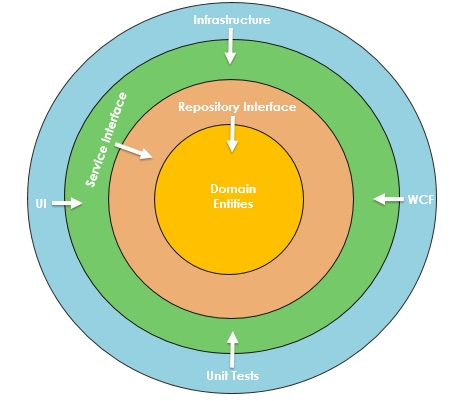
\includegraphics[width = 1\textwidth]{onion_architecture}
	\caption{Các lớp của Kiến trúc Onion}
\end{figure}

\textbf{Domain Layer - Lớp tên miền}

Ở phần trung tâm của Kiến trúc Onion, lớp miền tồn tại; lớp này đại diện cho các đối tượng nghiệp vụ và hành vi. Ý tưởng là có tất cả các đối tượng miền của bạn ở cốt lõi này. Nó chứa tất cả các đối tượng miền ứng dụng. Bên cạnh các đối tượng miền, bạn cũng có thể có các giao diện miền. Các thực thể miền này không có bất kỳ phụ thuộc nào.

\textbf{Repository Layer - Lớp kho lưu trữ}

Lớp này tạo ra một sự trừu tượng giữa các thực thể miền và logic nghiệp vụ của một ứng dụng. Trong lớp này, thường thêm các giao diện cung cấp hành vi lưu và truy xuất đối tượng thường bằng cách liên quan đến cơ sở dữ liệu. Lớp này bao gồm mẫu truy cập dữ liệu, là một cách tiếp cận kết hợp lỏng hơn để truy cập dữ liệu. Chúng tôi cũng tạo một kho lưu trữ chung và thêm các truy vấn để truy xuất dữ liệu từ nguồn, ánh xạ dữ liệu từ nguồn dữ liệu sang một thực thể kinh doanh và duy trì những thay đổi trong thực thể kinh doanh đối với nguồn dữ liệu.

\textbf{Services Layer - Lớp dịch vụ}

Lớp Dịch vụ giữ các giao diện với các hoạt động phổ biến, chẳng hạn như Thêm, Lưu, Chỉnh sửa và Xóa. Ngoài ra, lớp này được sử dụng để giao tiếp giữa lớp UI và lớp kho lưu trữ. Lớp Dịch vụ cũng có thể giữ logic nghiệp vụ cho một thực thể. Trong lớp này, các giao diện dịch vụ được giữ riêng biệt với quá trình triển khai của nó, giữ cho sự liên kết lỏng và tách biệt các mối quan tâm trong tâm trí.

\textbf{UI Layer - Lớp giao diện người dùng}

Đây là lớp ngoài cùng và giữ các mối quan tâm ngoại vi như giao diện người dùng và các thử nghiệm. Đối với một ứng dụng Web, nó đại diện cho dự án Web API hoặc Unit Test. Lớp này có sự triển khai của nguyên tắc tiêm phụ thuộc để ứng dụng xây dựng một cấu trúc liên kết lỏng và có thể giao tiếp với lớp bên trong thông qua các giao diện.

\subsection{Kiến trúc mô-đun}

Kiến trúc mô-đun (Modular Architecture) là kiểu kiến trúc phần mềm cho phép quản lý sự phức tạp của một vấn đề bằng cách chia nhỏ chúng thành các mô-đun để dễ quản lý hơn với các nguyên tắc và mô hình. Mô-đun là một đơn vị phần mềm không trạng thái có thể triển khai, quản lý, tái sử dụng, kết hợp lại và cung cấp giao diện ngắn gọn cho người dùng.

Khi phát triển phần mềm, khi hệ thống càng lớn thì càng cần thêm nhiều component, dẫn tới sự thay đổi nhỏ trong một component có thể ảnh hưởng tới nhiều component khác. Trong hệ thống, module là những component được phát triển bên ngoài ứng dụng. Module giao tiếp với ứng dụng thông qua entry-point.

\begin{figure}[ht]
	\centering
	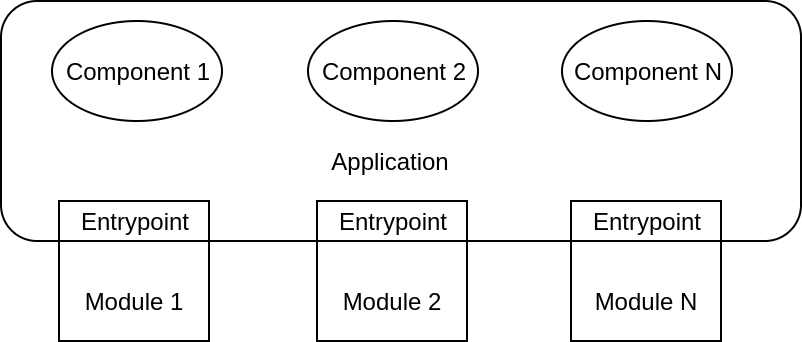
\includegraphics[width = 1\textwidth]{modules}
	\caption{Kiến trúc mô-đun}
\end{figure}

Sử dụng kiến trúc mô-đun đem lại một số lợi ích:

\begin{itemize}
	\bfitem{Tùy chỉnh}{ứng dụng có thể hoạt động thực sự khác biệt bằng cách chỉ bật / tắt một số mô-đun.}
	\bfitem{Ít phụ thuộc hơn}{các mô-đun độc lập hơn với chính ứng dụng, cho đến khi các "điểm vào" tương thích, cả mô-đun và ứng dụng có thể phát triển độc lập.}
	\bfitem{Các phần mở rộng của bên thứ ba}{vì các mô-đun không phải là một phần của ứng dụng và các "điểm vào" được xác định rõ, việc phát triển các mô-đun có thể được thực hiện bởi các bên thứ ba.}
	\bfitem{Phát triển độc lập}{Vì ứng dụng và các mô-đun là độc lập, chúng có thể là:}
	\begin{itemize}
		\item được phát triển bởi các nhà phát triển bên ngoài
		\item phát hành với các chu kỳ phát hành độc lập
		\item được phát triển tiềm năng với các công nghệ khác nhau
	\end{itemize}
	\bfitem{Ứng dụng nhỏ hơn}{Các ứng dụng nhỏ hơn (nhiều chức năng có thể được thực hiện thông qua các mô-đun) và ứng dụng nhỏ hơn được dịch để có khả năng bảo trì tốt hơn.}
\end{itemize}

Mô-đun được hình thành dựa trên việc nhóm những lớp có mức độ liên quan cao thành một mô-đun để có tính tương liên cao nhất. Có 2 loại tương liên:

\begin{itemize}
	\item Tương liên giao tiếp: có được khi 2 phần của mô-đun thao tác trên cùng dữ liệu.
	\item Tương liên chức năng: có được khi mọi phần của mô-đun làm việc cùng nhau để thực hiện tác vụ định rõ.
\end{itemize}

\section{Kiến trúc tổng quan hệ thống}

\subsection{Hệ thống frontend}

\subsubsection{Khởi tạo A/B Test}

\subsubsection{Kết quả A/B Test}

\subsection{Hệ thống backend}

\subsubsection{Khởi tạo A/B Test}

\subsubsection{Thực hiện A/B Test}

\subsubsection{Đánh giá A/B Test}

\subsection{Biểu đồ tuần tự}

\subsubsection{Khởi tạo A/B Test}

\subsubsection{Thực hiện A/B Test}

\subsubsection{Đánh giá A/B Test}

\section{Mô hình cơ sở dữ liệu}

\subsection{Mô hình quản lý A/B Test}

\subsection{Mô hình theo dõi kết quả}

\subsection{Mô hình phân bố dữ liệu}
